\documentclass[12pt]{article}
\pagestyle{empty}
\usepackage{graphicx}
\usepackage{amsmath}
\usepackage{amsfonts}

\title{Nonlinear FEM Homework 1}
\author{Truman Ellis}
\date{}

\begin{document}
\paragraph{b)}
Plots of shape functions for $h=0.5$.
\begin{figure}[h!]
\centering
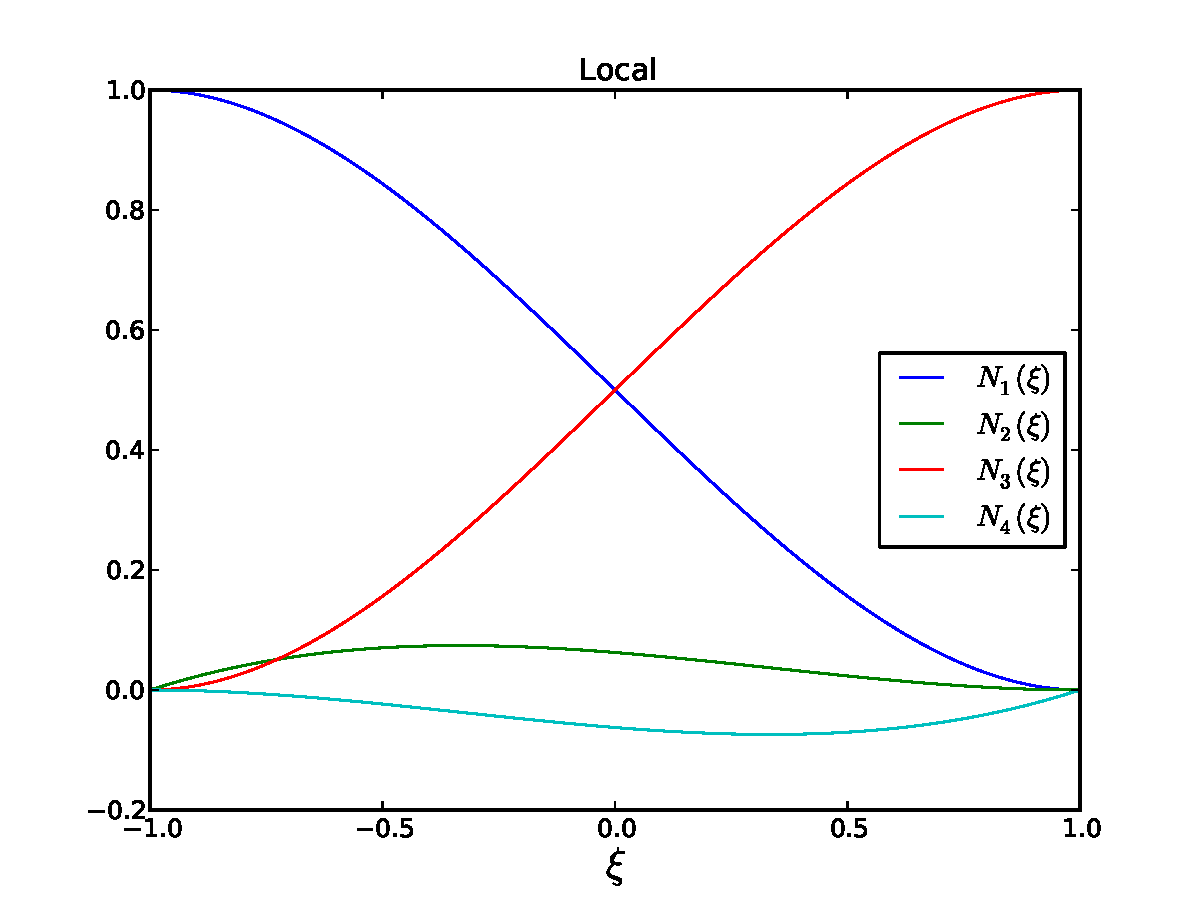
\includegraphics[width=0.8\textwidth]{Local.pdf}
\end{figure}
\begin{figure}[h!]
\centering
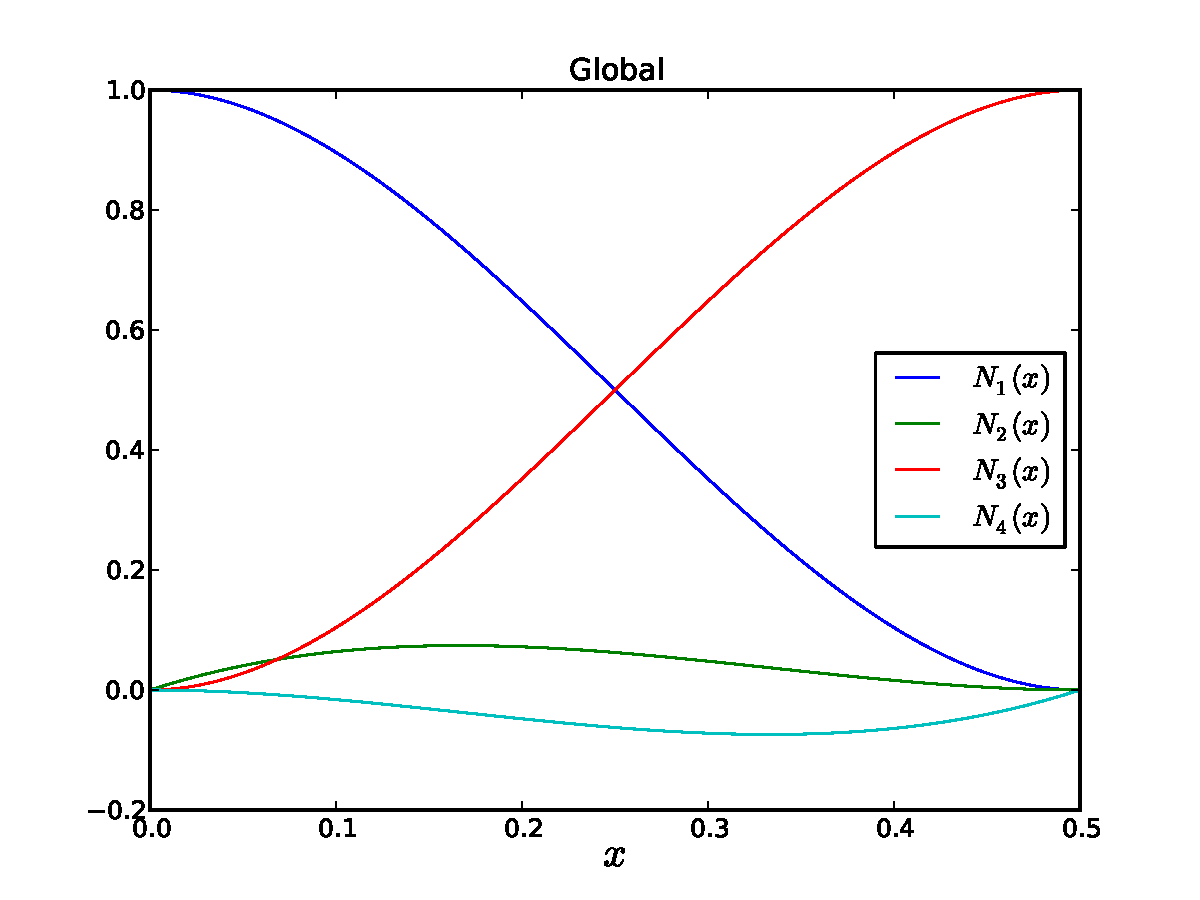
\includegraphics[width=0.8\textwidth]{Global.pdf}
\end{figure}

\paragraph{f)}

Results for $c=1$, $M=Q=0$.
\begin{figure}[h!]
\centering
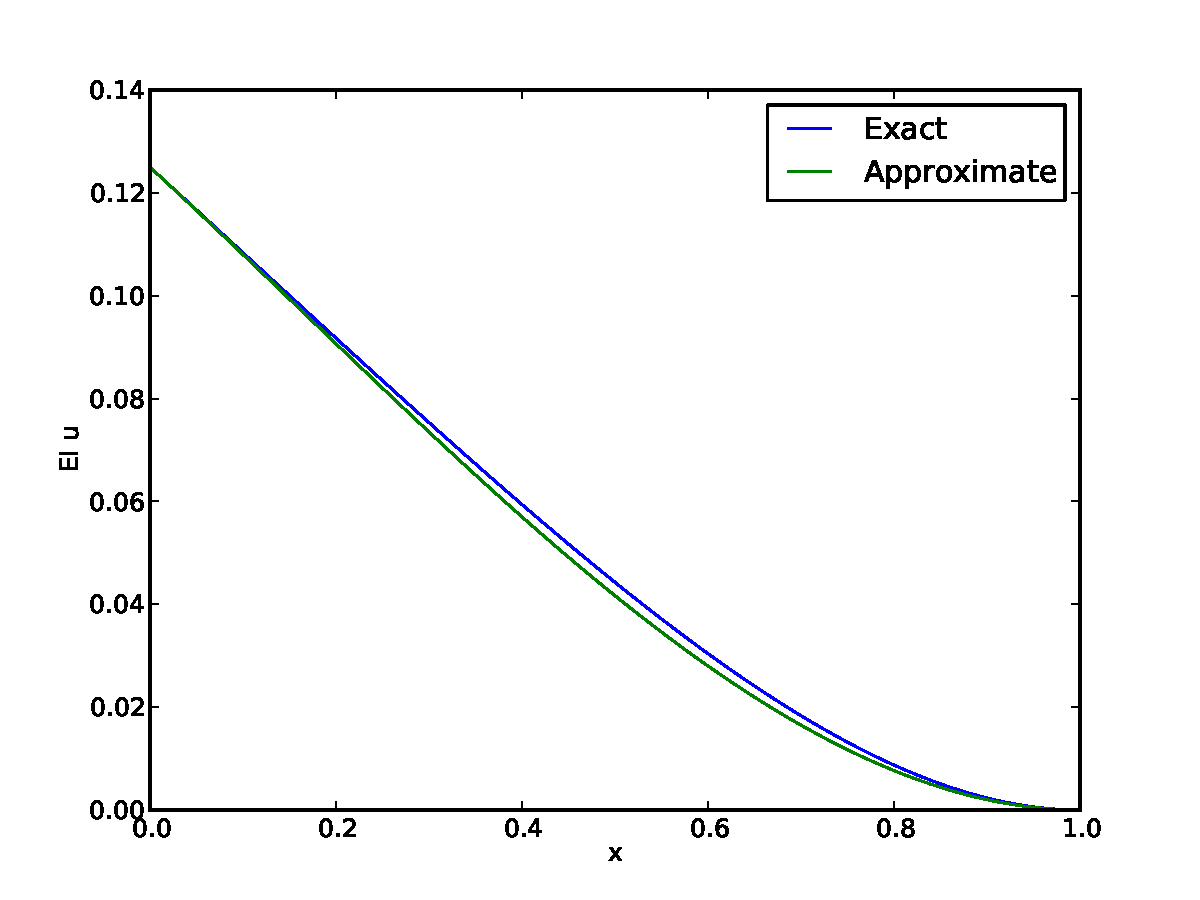
\includegraphics[width=0.9\textwidth]{u.pdf}
\end{figure}
\begin{figure}[h!]
\centering
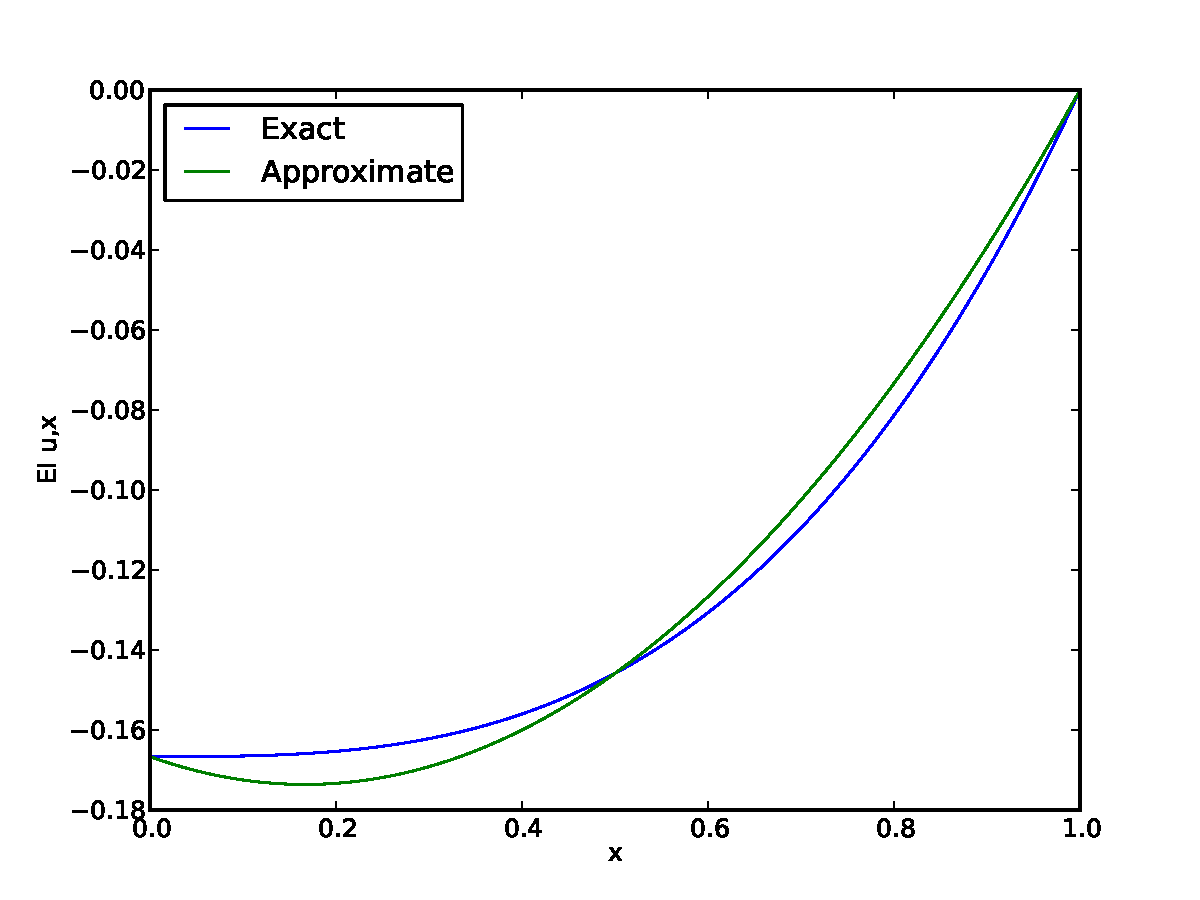
\includegraphics[width=0.9\textwidth]{ux.pdf}
\end{figure}
\begin{figure}[h!]
\centering
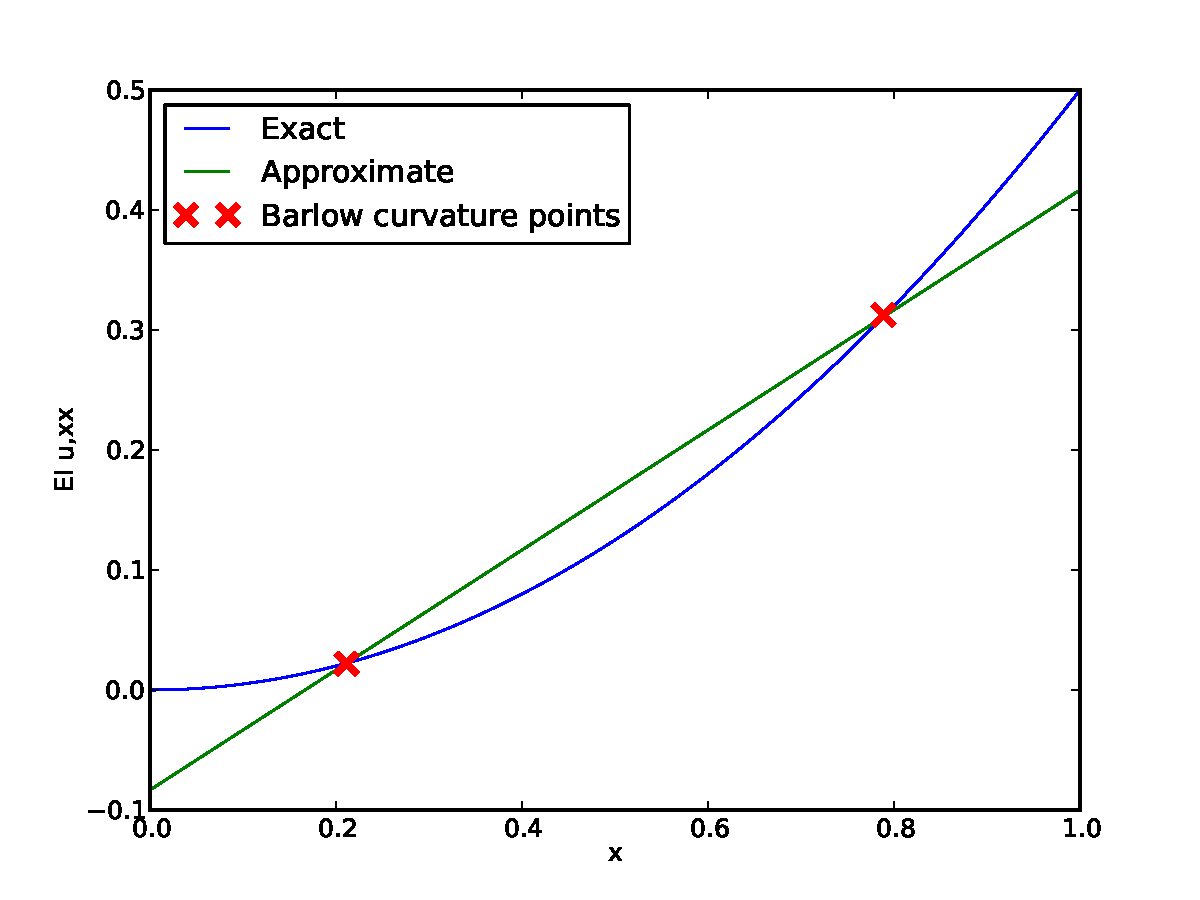
\includegraphics[width=0.9\textwidth]{uxx.pdf}
\end{figure}

\clearpage
Results for $c=10$, $M=Q=-5$.
\begin{figure}[h!]
\centering
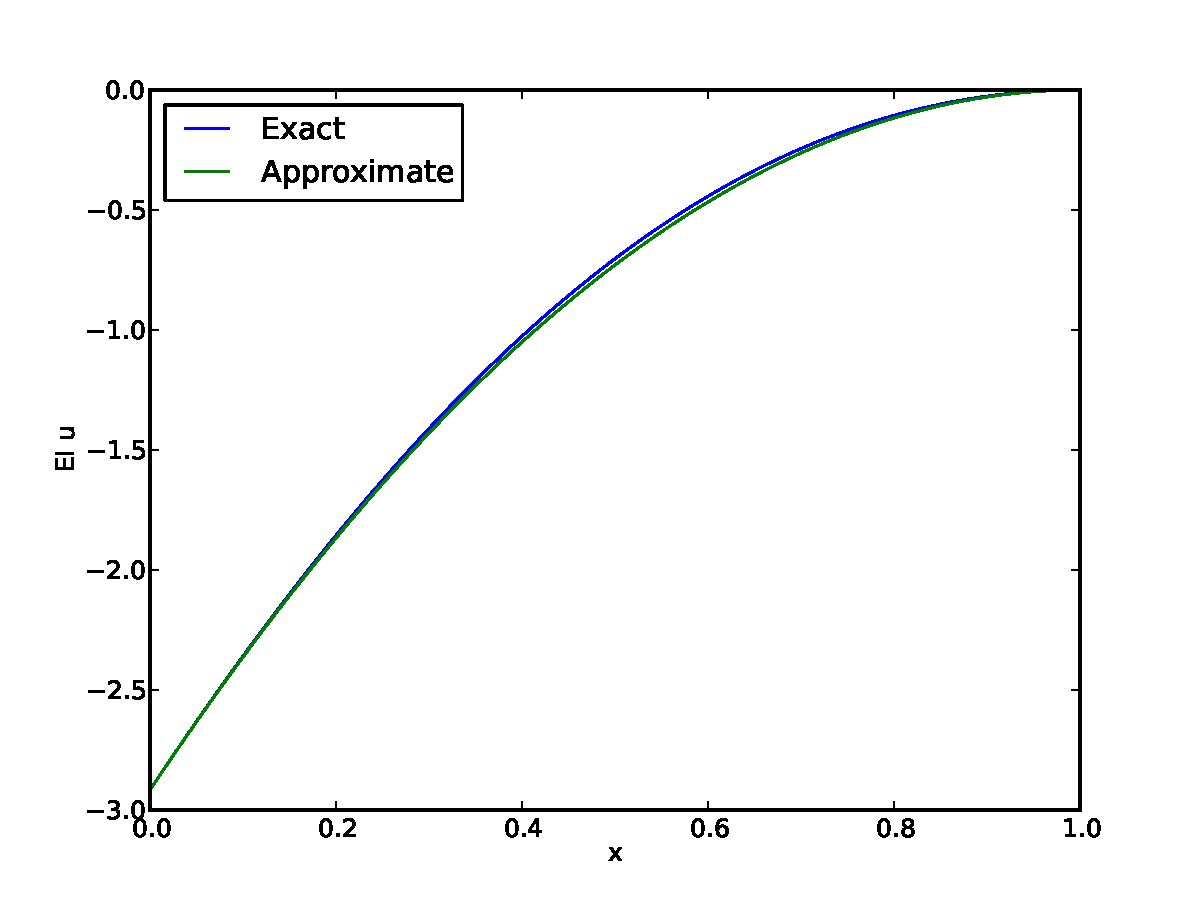
\includegraphics[width=0.9\textwidth]{u1.pdf}
\end{figure}
\begin{figure}[h!]
\centering
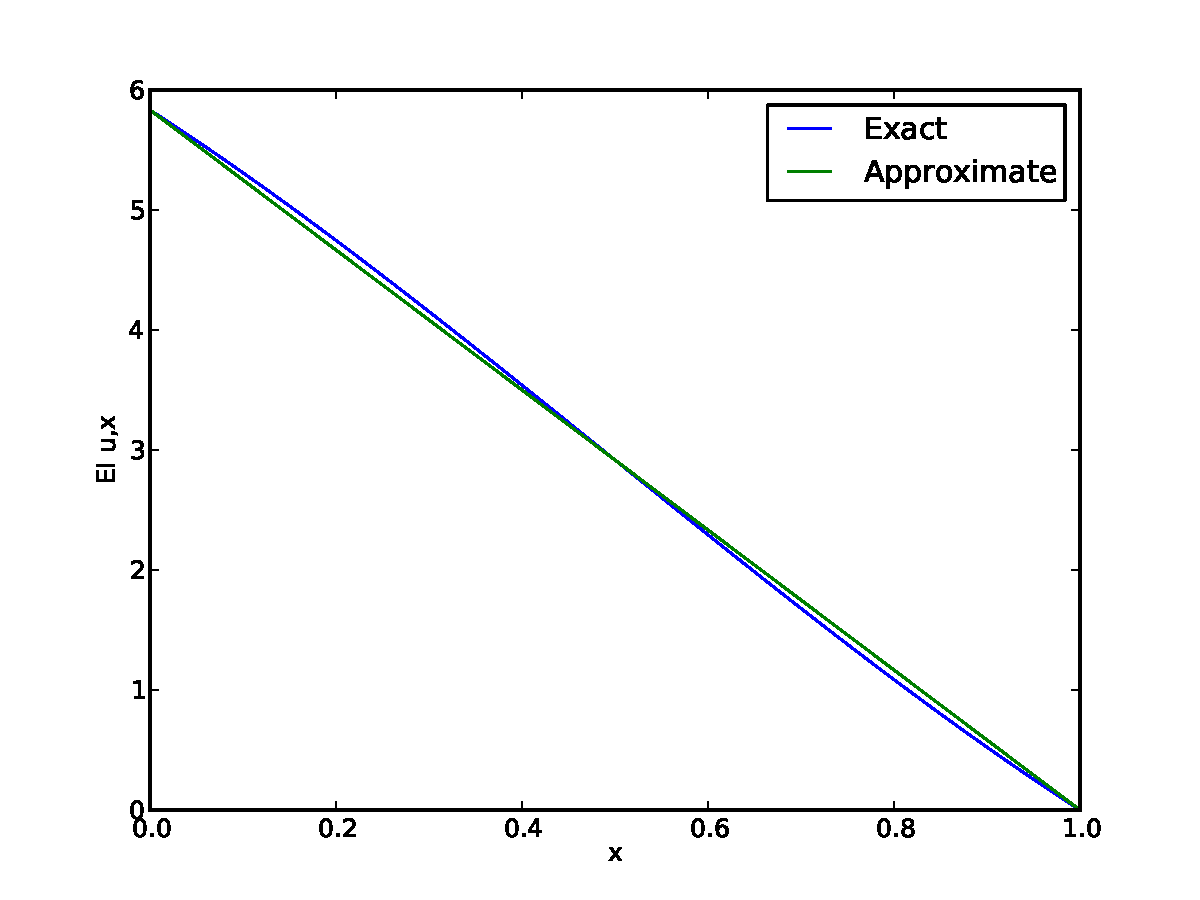
\includegraphics[width=0.9\textwidth]{ux1.pdf}
\end{figure}
\begin{figure}[h!]
\centering
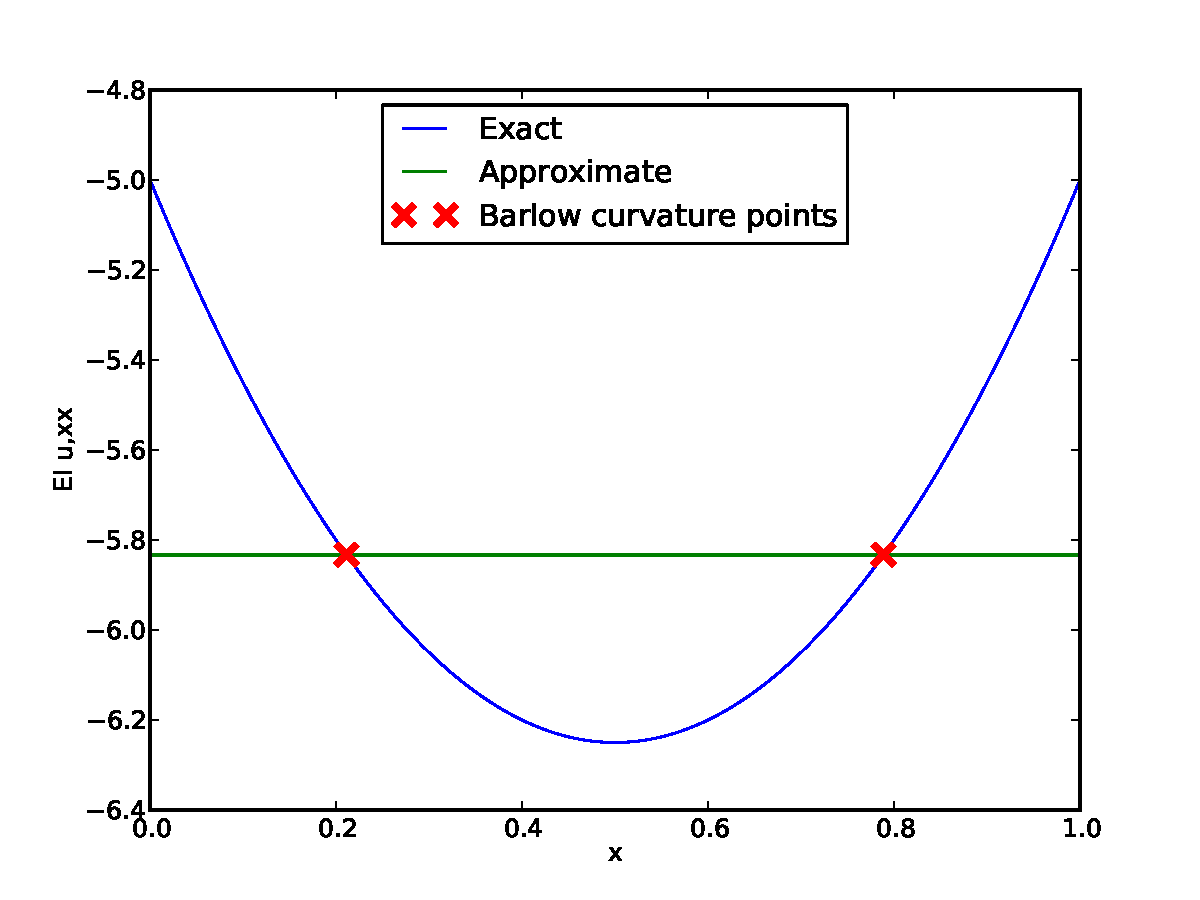
\includegraphics[width=0.9\textwidth]{uxx1.pdf}
\end{figure}
% \maketitle
% 
% $\Omega=(0,1)$
% \paragraph{(S)}
% Given $f:\Omega\rightarrow\mathbb{R}$ and constants $M$ and $Q$, find
% $u:\bar{\Omega}\rightarrow\mathbb{R}$ such that
% \begin{align*}
% EI u_{,xxxx}&=f\quad\text{ on }\Omega\\
% u(1)&=0\\
% u_{,x}(1)&=0\\
% EIu_{,xx}(0)&=M\\
% EIu_{,xxx}&=Q
% \end{align*}
% 
% Let $\mathcal{S}=\mathcal{V}=\left\{w|w\in H^2(\Omega),
% w(1)=w_{,x}(1)=0\right\}$.
% 
% \paragraph{(W)}
% Given $f$, $M$, and $Q$, find $u\in\mathcal{S}$ such that $\forall
% w\in\mathcal{V}$
% \[
% a(w,u)=(w,f)-w_{,x}(0)M+w(0)Q
% \]
% where
% \[
% a(w,u)=\int_0^1w_{,xx}EIu_{,xx}dx
% \]
% \[
% (w,f)=\int_0^1wfdx
% \]
% 
% Let $\mathcal{S}^h=\mathcal{V}^h$ be a finite dimensional approximation of
% $\mathcal{S}$.
% 
% \paragraph{(G)}
% Given $f$, $M$, and $Q$, find $u^h\in\mathcal{S}^h$ such that $\forall
% w^h\in\mathcal{V}^h$
% \[
% a(w^h,u^h)=(w^f,f)-w_{,x}^h(0)M+w^h(0)Q
% \]
% 
% \paragraph{a)} Assuming all functions are smooth and bounded, show that the
% solutions of (S) and (W) are identical. What are the natural boundary
% conditions?
% 
% Let $u$ be the solution of (S), then
% \[
% 0=-\int_0^1w(EIu_{,xxxx}-f)dx
% \]
% for any $w\in\mathcal{V}$.
% 
% Integrating by parts twice
% \begin{align*}
% 0&=\int_0^1EIw_{,x}u_{,xxx}dx+\int_0^1wfdx\underbrace{-EIwu_{,xxx}|_0^1}_{w(0)Q}\\
% &=-\int_0^1EIw_{,xx}u_{,xx}dx+\int_0^1wf+w(0)Q\underbrace{+EIw_{,x}u_{,xx}|_0^1}_{-w_{,x}(0)M}\\
% &=-a(w,u)+(w,f)-w_{,x}(0)M+w(0)Q
% \end{align*}
% Therefore $u$ solves (W).
% 
% Let $u$ be the solution of (W), then $w\in\mathcal{S}$ so $u(1)=u_{,x}(1)=0$.
% \[
% \int_0^1EIw_{,xx}u_{,xx}dx=\int_0^1wfdx-w_{,x}(0)M+w(0)Q \quad\forall
% w\in\mathcal{V}
% \]
% Integrating by parts twice using $w(1)=w_{,x}(1)=0$
% \begin{align*}
% &-\int_0^1EIw_{,x}u_{,xxx}dx+EIw_{,x}u_{,xx}|_0^1=(w,f)-w_{,x}(0)M+w(0)Q\\
% &\int_0^1EIwu_{,xxxx}dx+EIwu_{,xxx}|_0^1+EIw_{,x}(0)u,xx=(w,f)-u_{,x}(0)M+w(0)Q
% &0=\int_0^1w(EIu_{,xxxx}-f)dx+w(0)(EIu_{,xxx}(0)-Q)+EIw_{,x}(0)u,xx=(w,f)-u_{,x}(0)M+w(0)Q
% 
% \end{align*}

\end{document}
